\section{Laboratory Lecture 1: Stepper Motor Controller}

The aim of this laboratory session is to design a stepper motor controller using an ATMega328P microcontroller. Since the basics of stepper motors have already been covered in \textbf{Section \ref{sec:STEPPER_MOTOR}}, they will not be discussed again. However, a brief introduction to the ATMega328P is necessary to fully understand this laboratory session.

\subsection{Introduction}

The Atmel ATMega328P is an 8-bit, low-power CMOS 8-bit microcontroller based on the AVR enhanced RISC architecture. It is built around a Harvard architecture, which means that the Data Memory bus and the Program memory bus are different. In this specific case, it can be said that its data word size is 8 bits and its program word size is 16 bits.\medskip 

The AVR core combines a rich instruction set with 32 general purpose working registers. All the 32 registers are directly connected to the arithmetic logic unit (ALU), allowing two independent registers to be accessed in one single instruction executed in one clock cycle. The resulting architecture is more code efficient while achieving throughputs up to ten times faster than conventional CISC microcontrollers.\medskip

The Atmel ATMega328P provides the following features: 32K bytes of in-system programmable flash with read-while-write capabilities, 1K bytes EEPROM, 2K bytes SRAM, 23 general purpose I/O lines, 32 general purpose working registers, three flexible Timer/Counters with compare modes, internal and external interrupts, a serial programmable USART, a byte oriented 2-wire serial interface, an SPI serial port, a 6-channel 10-bit ADC (8 channels in TQFP and QFN/MLF packages), a programmable watchdog timer with internal oscillator, and five software selectable power saving modes. The idle mode stops the CPU while allowing the SRAM, Timer/Counters, USART, 2-wire serial interface, SPI port, and interrupt system to continue functioning. The power-down mode saves the register contents but freezes the oscillator, disabling all other chip functions until the next interrupt or hardware reset. In power-save mode, the asynchronous timer continues to run, allowing the user to maintain a timer base while the rest of the device is sleeping. The ADC noise reduction mode stops the CPU and all I/O modules except asynchronous timer and ADC, to minimize switching noise during ADC conversions. In standby mode, the crystal/resonator oscillator is running while the rest of the device is sleeping. This allows very fast start-up combined with low power consumption.\medskip

The device is manufactured using Atmel high density non-volatile memory technology. The on-chip ISP flash allows the program memory to be reprogrammed in-system through an SPI serial interface, by a conventional non-volatile memory programmer, or by an on-chip boot program running on the AVR core. The boot program can use any interface to download the application program in the application flash memory. Software in the boot flash section will continue to run while the application flash section is updated, providing true read-while-write operation. By combining an 8-bit RISC CPU within-system self-programmable flash on a monolithic chip, the Atmel ATmega328P is a powerful microcontroller that provides a highly flexible and cost effective solution to many embedded control applications.\medskip

The ATMega328P AVR is supported with a full suite of programs and system development tools including: C compilers, macro assemblers, program debugger/simulators, in-circuit emulators, and evaluation kits.~\autocite{ATMEGA328P}\medskip

A diagram describing its pinout can be found below:

\begin{figure}[H]
    \centering
    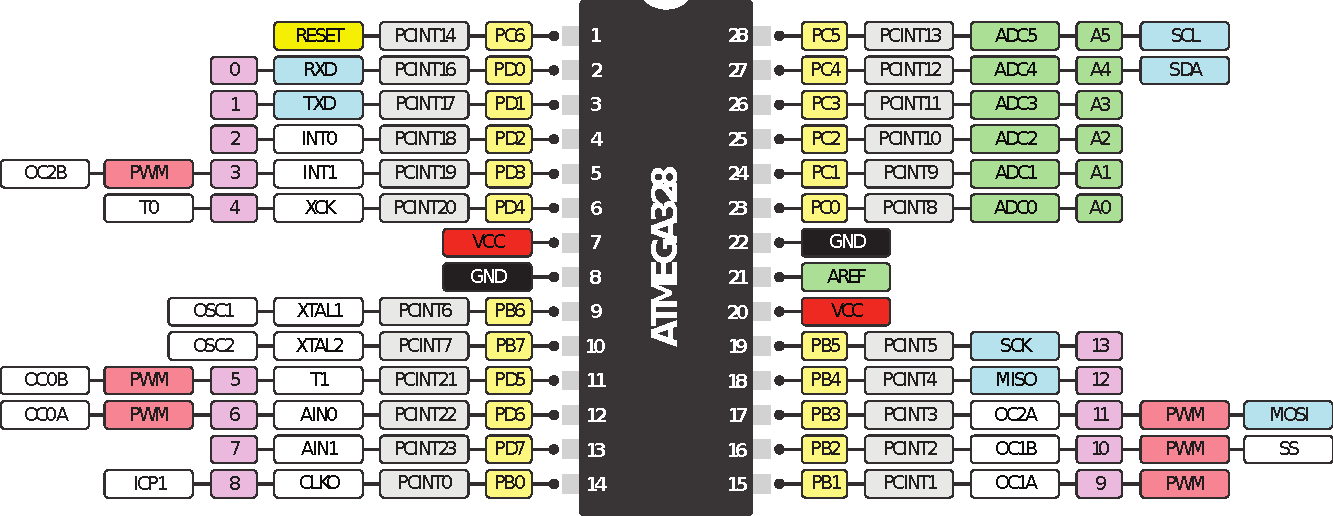
\includegraphics[scale = 0.55]{Graphics/MICROS/Practice 1/ARDUINO/ATMEGA328P_PINOUT.pdf}
    \caption{ATMega328p's Pinout~\autocite{ATMEGA328P_PINOUT}}
    \label{fig:ATMEGA328P_PINOUT}
\end{figure}


\subsection{Arduino}
\label{sec:ARDUINO}

The popularity of the ATMega328P can be attributed to its use in the Arduino development board, the design of which falls within the Open Source Hardware category/movement. For our designs, as well as for real-life testing, we will use this board, in particular the Arduino UNO, which breaks out most of the pins into headers, supplies the ATMega with a stable voltage and provides native USB communication.\medskip

\clearpage

A diagram of the Arduino UNO board can be found below:

\begin{figure}[H]
    \centering
    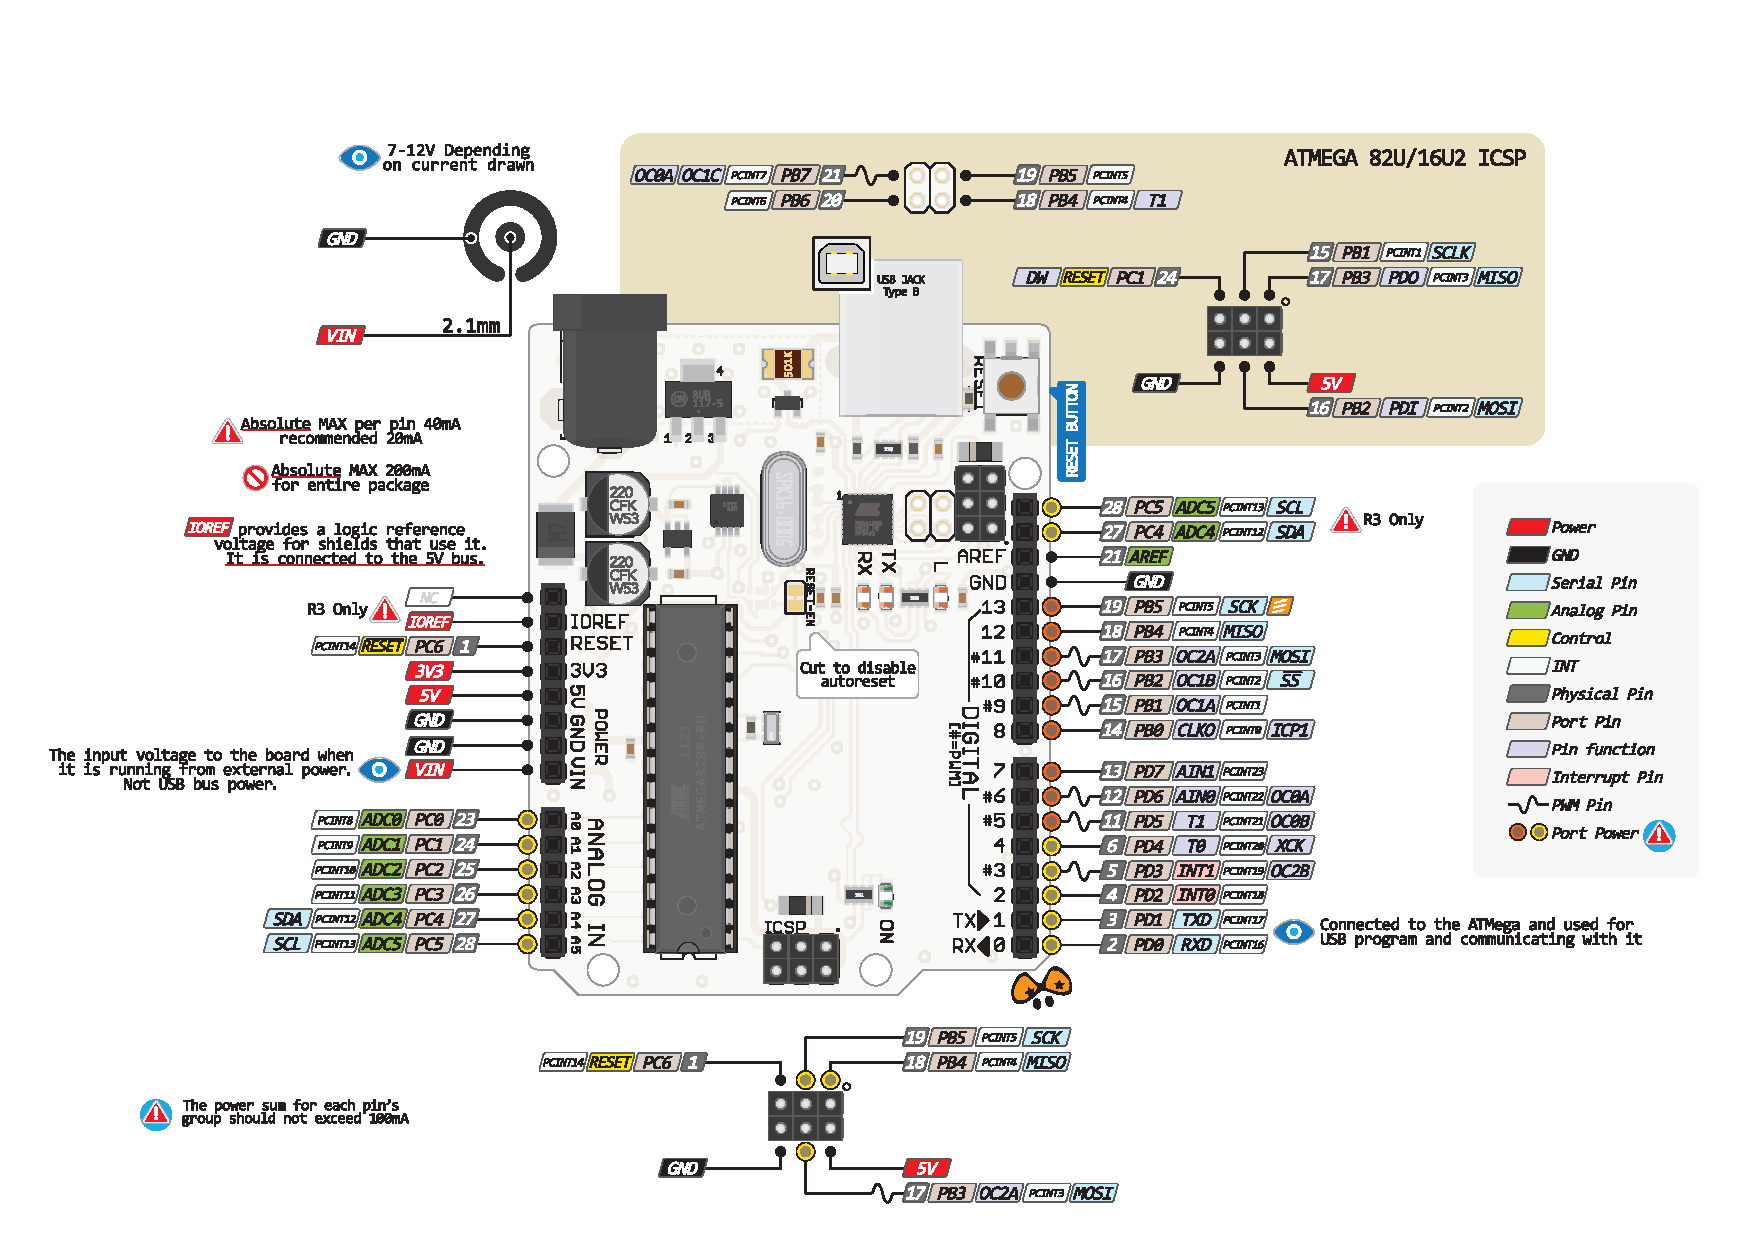
\includegraphics[scale = 0.50]{Graphics/MICROS/Practice 1/ARDUINO/BOARD.pdf}
    \caption{Arduino UNO Pinout~\autocite{BQ_ARDUINO}}
    \label{fig:ARDUINO_UNO_BOARD}
\end{figure}

\subsection{I/O Ports}

The I/O ports allow the user to communicate with the ATMega. All AVR ports, in general, can be said to have have true Read-Modify-Write functionality when used as general digital I/O ports. This means that the direction of one port pin can be changed without unintentionally changing the direction of any other pin.\medskip

The ATMega328P has 3 8-bit ports, namely B, C, D. Each port is controlled by three 8-bit registers:

\begin{enumerate}
    \item \textbf{DDRx -} Direction Register
        \begin{itemize}
            \item Defines wheter a pin in as input (0) or an output (1)
        \end{itemize}
    \item \textbf{PINx -} Pin Input Value Register
        \begin{itemize}
            \item Reading this register bit returns the value of the specific pin.
        \end{itemize}
    \item \textbf{PORTx - } Pin Output Value Register
        \begin{itemize}
            \item Writing to this register SETS the value of a pin.
        \end{itemize}
\end{enumerate}

\clearpage

The internal circuit that controls the state of each pin can be seen below:

\begin{figure}[H]
    \centering
    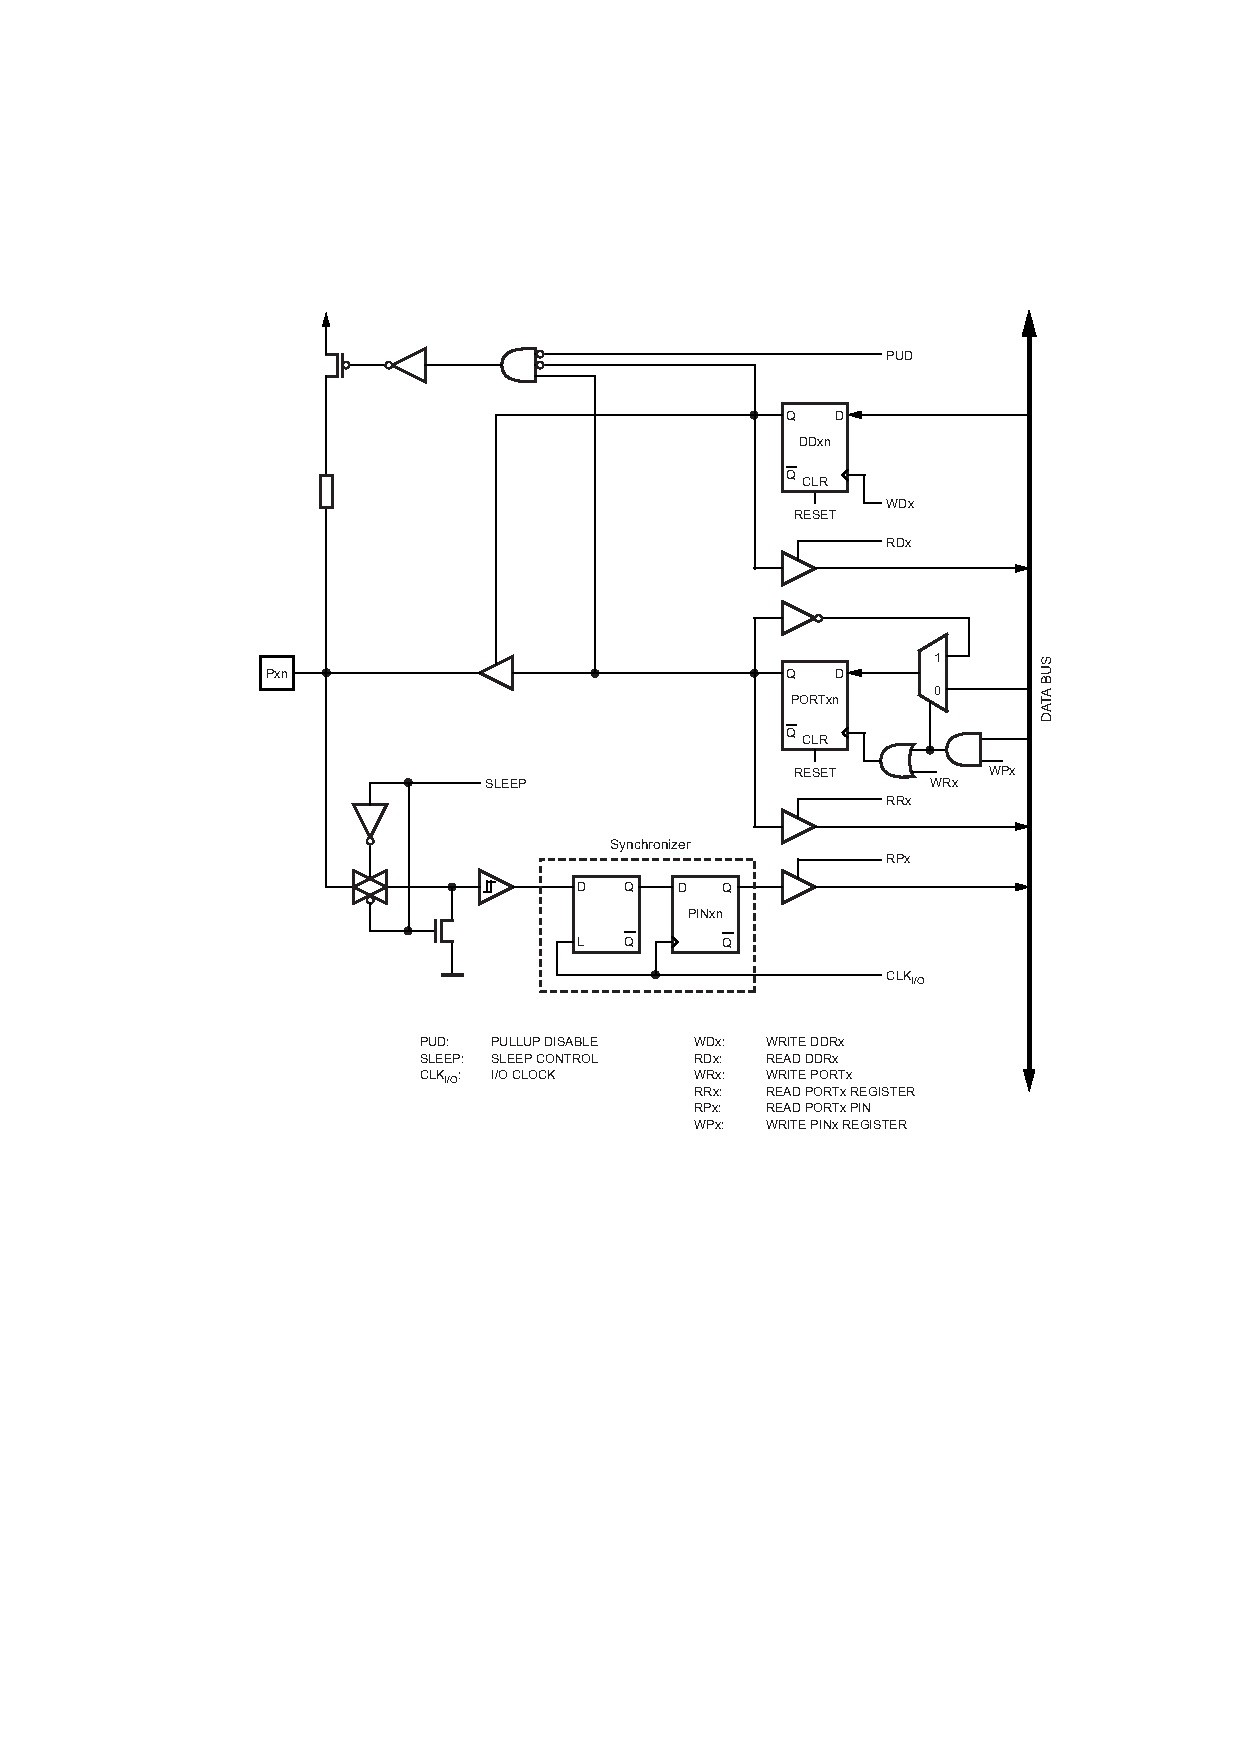
\includegraphics[scale = 0.9]{Graphics/MICROS/Practice 1/ARDUINO/INTERNAL_PIN_SETTING.pdf}
    \caption{Internal I/O individual control circuit~\autocite{ATMEGA328P}}
    \label{fig:I/O_CONTROL}
\end{figure}


To interact with the 3 mentioned ports, some information regarding the registers, DDRx, PINx, and PORTx, must be known. This information can be found in the datasheet~\autocite{ATMEGA328P}.\medskip

Attached below is an example of all of the registers bound to PORTB.

\begin{figure}[H]
    \centering
    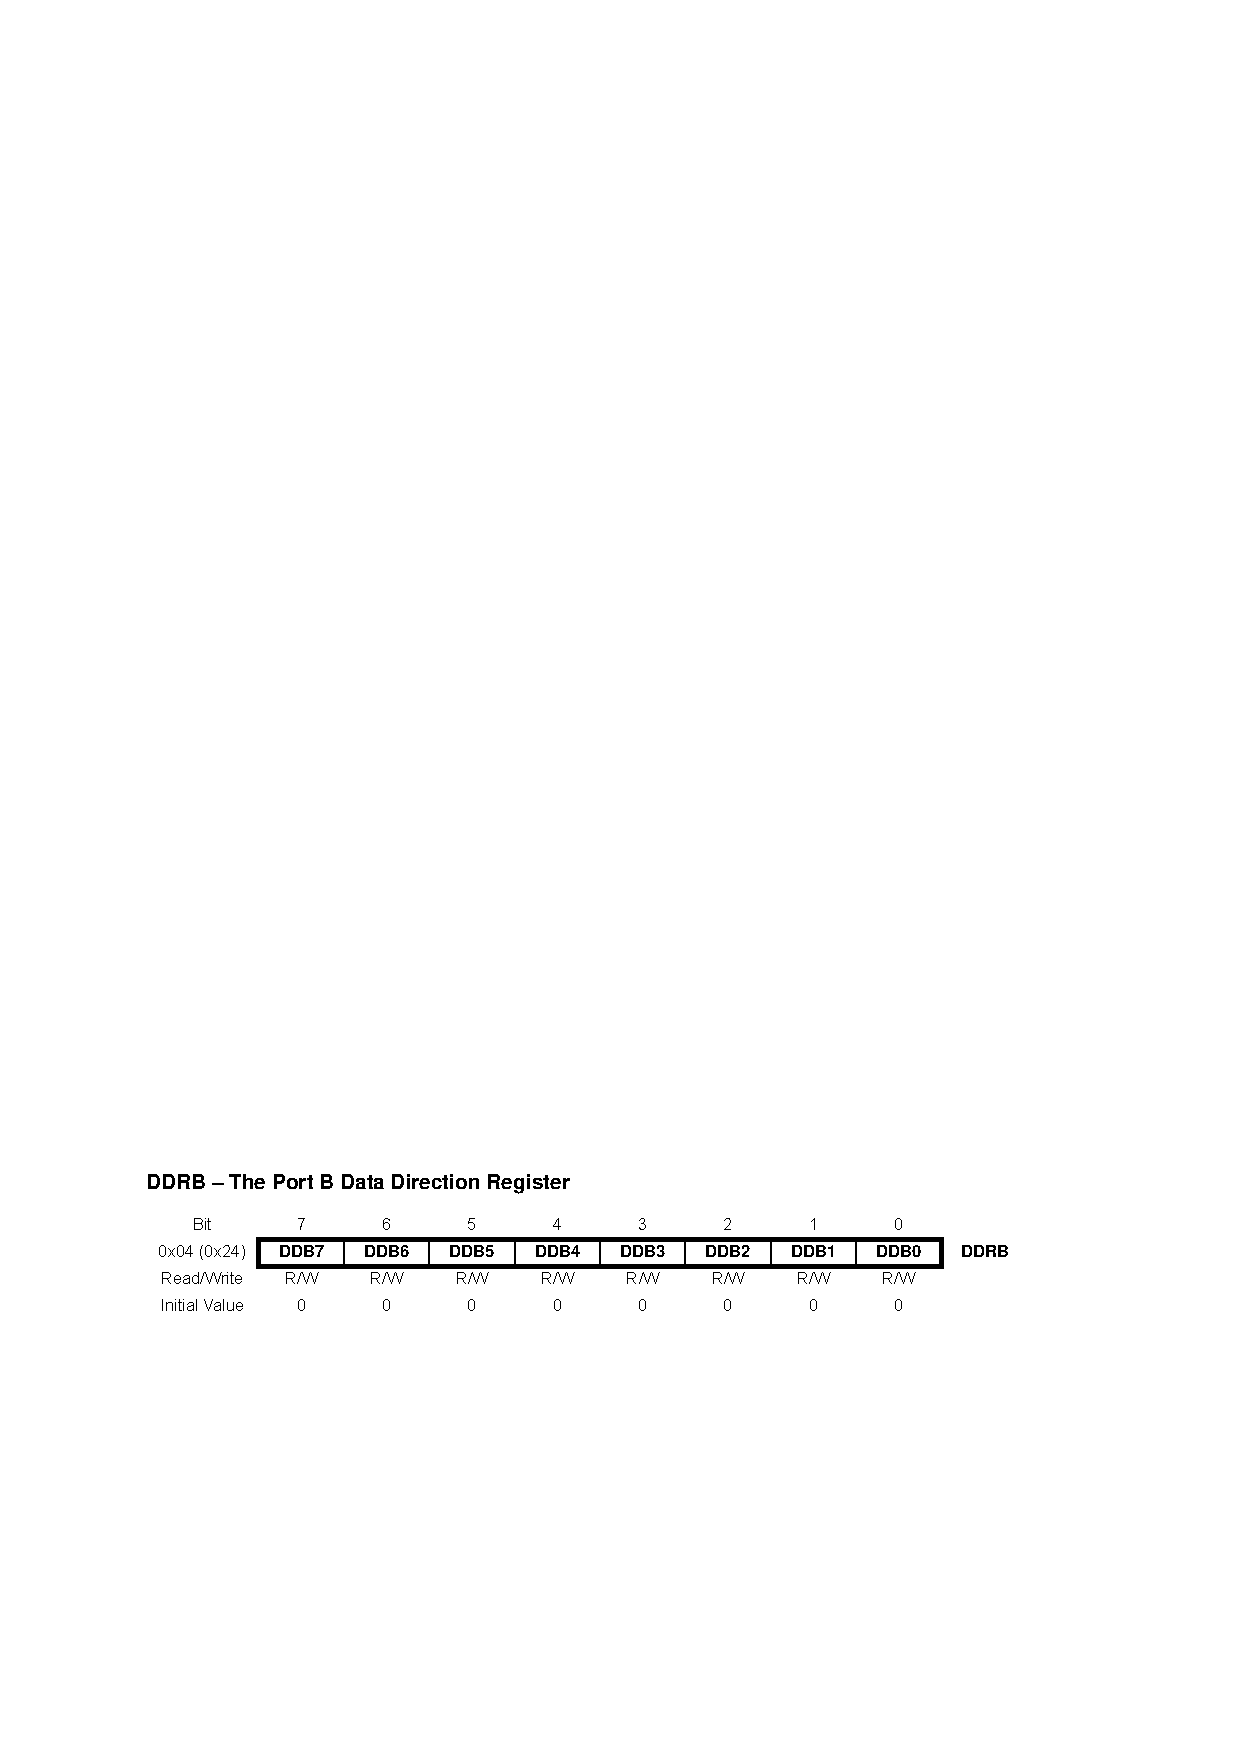
\includegraphics[width = \textwidth]{Graphics/MICROS/Practice 1/DATSHEET/DDRB.pdf}
    \caption{DDRB - Direction Register B (Used to set pins as I/O)}
    \label{fig:DDRB}
\end{figure}

\begin{figure}[H]
    \centering
    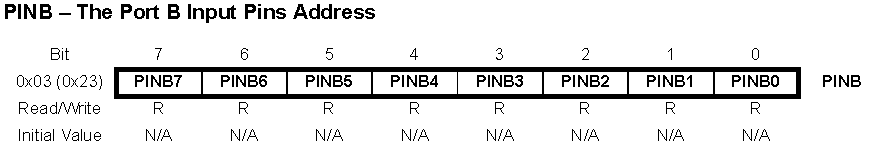
\includegraphics[width = \textwidth]{Graphics/MICROS/Practice 1/DATSHEET/PINB.pdf}
    \caption{PINB - PORTB Input Pins Address (Used to read the value of an specific pin)}
    \label{fig:PINB}
\end{figure}

\begin{figure}[H]
    \centering
    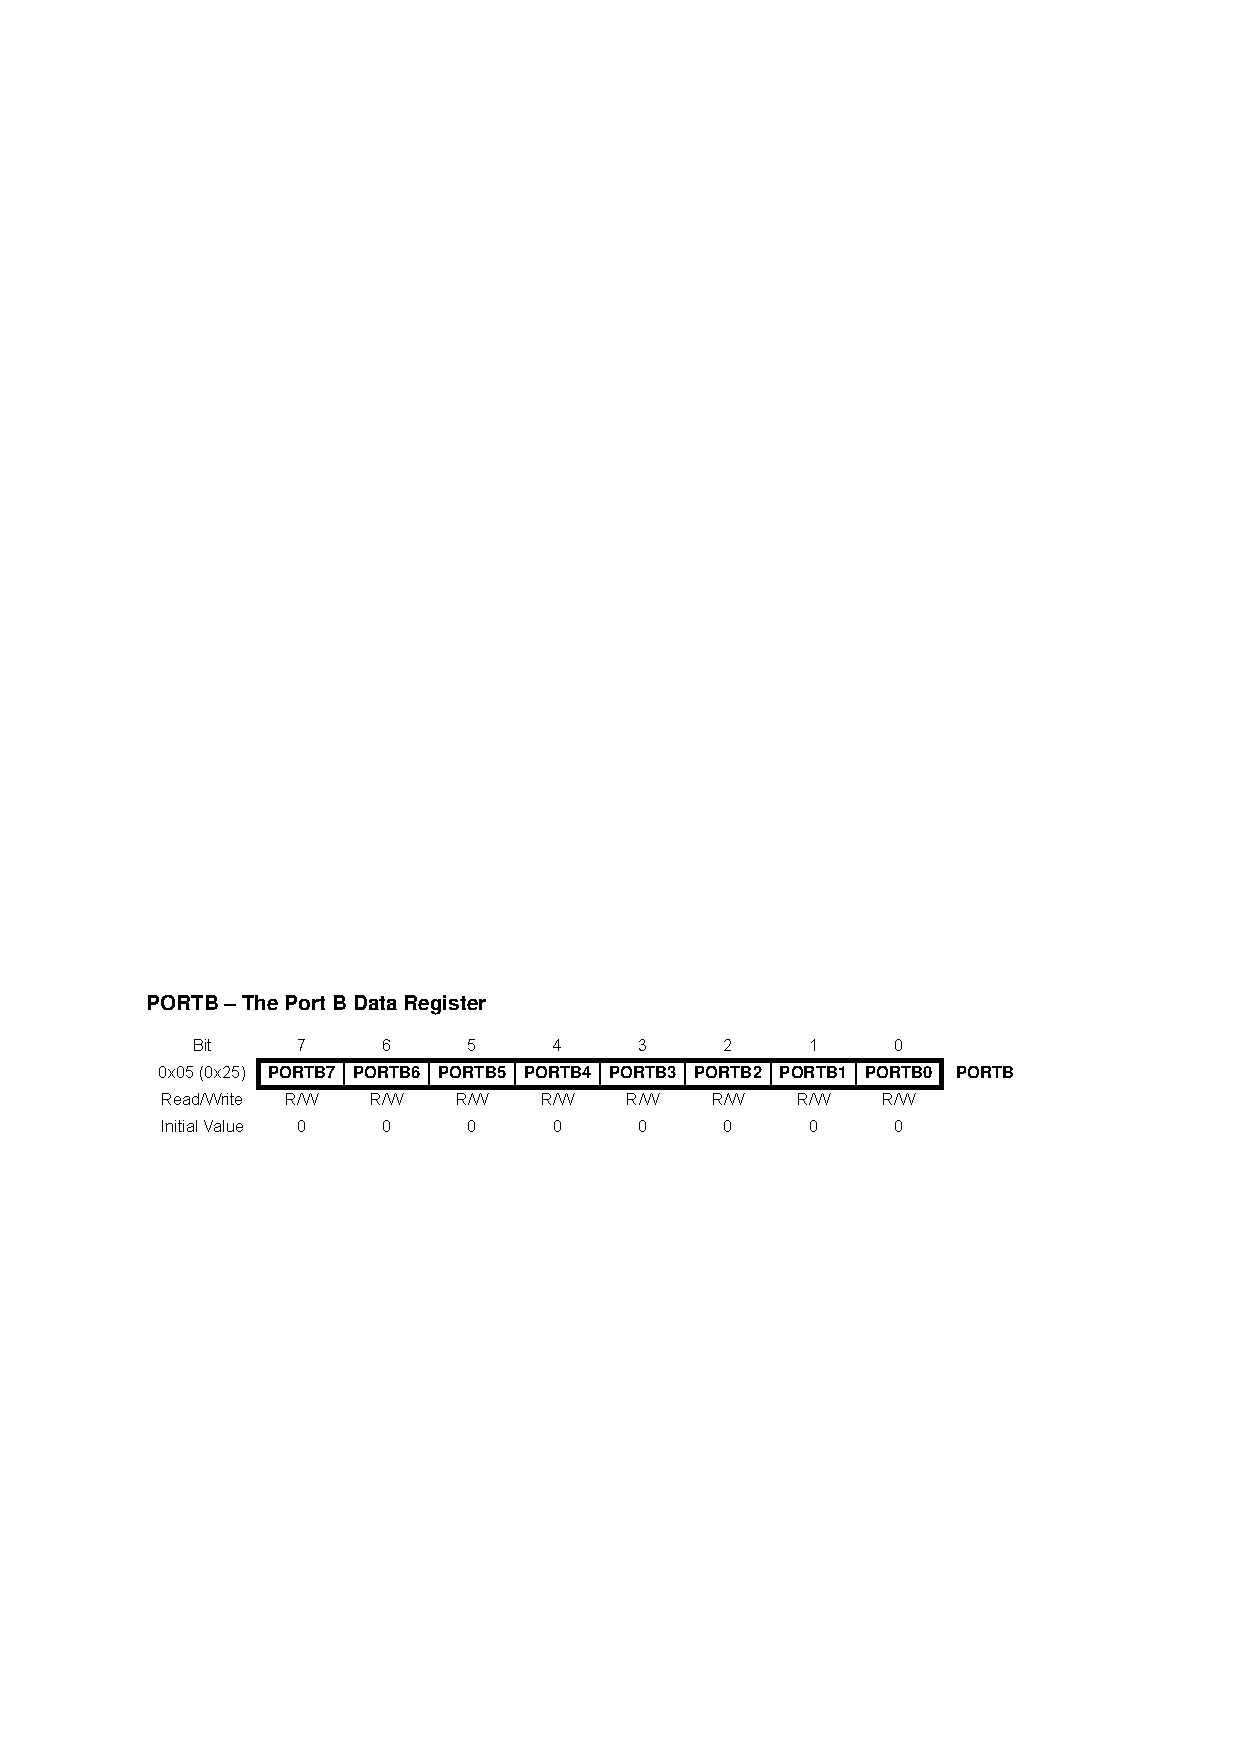
\includegraphics[width = \textwidth]{Graphics/MICROS/Practice 1/DATSHEET/PORTB.pdf}
    \caption{PORTB - PORTB Data Register (Used to set the Output value and the pull-ups)}
    \label{fig:PORTB}
\end{figure}

We can also find an addional register called \textit{MCUCR} in the datasheet. Setting its PUD bit (bit 4) to 1, will disable the pull-ups, even if the DDxn and the PORTxn registers are configured to enable them. 

\begin{figure}[H]
    \centering
    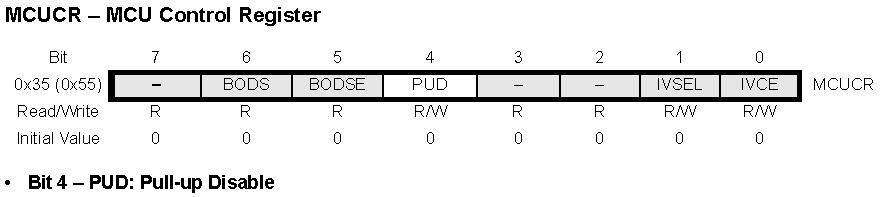
\includegraphics[width = \textwidth]{Graphics/MICROS/Practice 1/DATSHEET/MCUCR.pdf}
    \caption{MCUCR – MCU Control Register}
    \label{fig:MCUR}
\end{figure}


By changing the state of the corresponing bits of each of the three registers, the behaviour if the pin can be changed. The possible combinations are listed below:


\begin{table}[htbp]
    \resizebox{\columnwidth}{!}{
        \centering
        \begin{tabular}[t]{lcccccc}
            \toprule
            & \textbf{DDxn} & \textbf{PORTxn} & \textbf{PUD (in MCUCR)} & \textbf{I/O} & \textbf{Pull-up} & \textbf{Comment}\\
            \midrule
            & 0 & 0 & X & Input  & No  & Tri-state (Hi-Z)                            \\
            & 0 & 1 & 0 & Input  & Yes & Source current if pulled low  \\
            & 0 & 1 & 1 & Input  & No  & Tri-state (Hi-Z)                            \\
            & 1 & 0 & X & Output & No  & Output Low (Sink)                           \\
            & 1 & 1 & X & Output & No  & Output High (Source)                        \\
            \bottomrule
        \end{tabular}
        \caption{Available Pin Modes.~\autocite{ATMEGA328P}}
        \label{table:PIN_MODES}
        }
\end{table}


\clearpage

\subsection{C Applied to Microcontrollers}

To program the ATMega328P, as well as most microcontrollers, we will use C. C offers the benefit of being a high-level language, i.e., it is nos as hard to understand as Machine code or Assembly. Even though programming in C or in other high-level languages is not as efficient as directly programming in Assembly, since it has to go though a compiles, its simplicity normally outweights the decrease in code efficiency. \medskip

We will now go over the basics of writing and reading to the registers that have been previously mentioned.


\subsubsection{Reading from an I/O Register}

To read from a register, we can simply access them as if we were reading a variable.

\inputCcode{CODES/MICROS/Practice_1/EXPLANATION/READING_REG.c}

Reading the value of a specific byte can be done in two ways:

\inputCcode{CODES/MICROS/Practice_1/EXPLANATION/READING_BIT_NATIVE.c}

Which is basically C syntax.

\inputCcode{CODES/MICROS/Practice_1/EXPLANATION/READING_BIT_BUILTIN.c}

Which does the same thing but in a non-C-standard way.

\clearpage

\subsubsection{Writing to an I/O Register}

To write to a whole register, we can access it as if we were assigning a value to a variable:

\inputCcode{CODES/MICROS/Practice_1/EXPLANATION/WRITING_REG.c}

To write to a specific bit beloging to any of the registers we do:

\inputCcode{CODES/MICROS/Practice_1/EXPLANATION/WRITING_BIT_ONE.c}

Multiple bits can be written to at the same time as well:

\inputCcode{CODES/MICROS/Practice_1/EXPLANATION/WRITING_BIT_SEVERAL.c}

\clearpage

\subsection{Exercise 1: Stepper Motor Controller}

Now that we have established the basics, it is time to move on to solving the proposed exercise. As we saw in \textbf{Section \ref{sec:STEPPER_MOTOR}}, a stepper motor can be controlled using three methods, namely, Full-Step, Half-Step, and Wave-Step.\medskip 

In this practice we will only focus on the first method, as the others are very similar and do not pose more of a challenge than the first one.\medskip

The main objective of this practice is to control the direction of rotation of a stepper motor. In order to do this, we will use an L293D driver IC, as we saw in previous sections. By changing the state of a switch, the ATMega328P, will reverse the order of the Full-Step sequence shown in \textbf{Table \ref{table: PHASE_CURRENT_WAVEFORMS}}, effectively reversing the spin of the motor.\medskip

A block diagram describing the operation of the code can be seen below:

\begin{figure}[H]
    \centering
    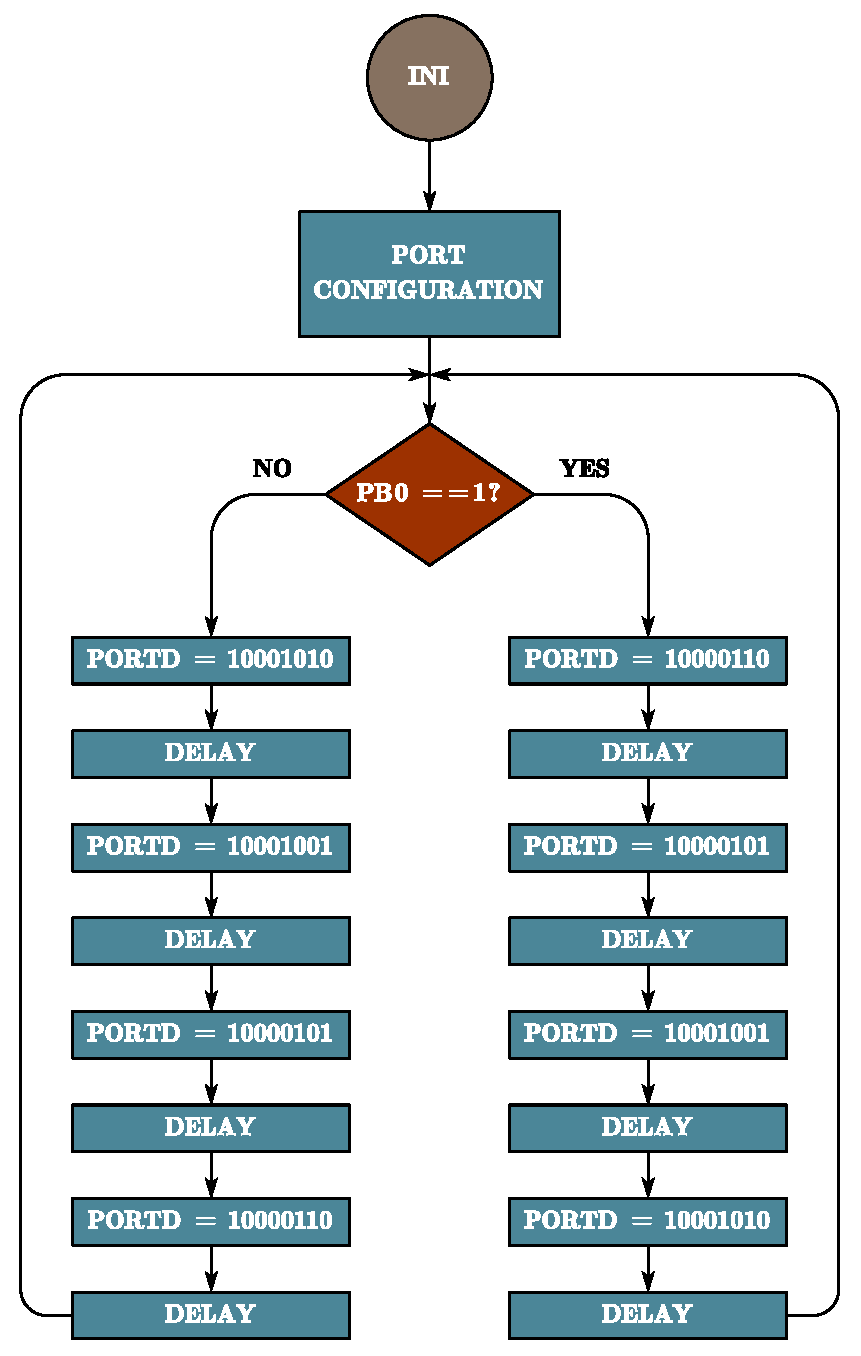
\includegraphics[scale = 0.6]{Graphics/MICROS/Practice 1/BLOCK-DIAGRAM.pdf}
    \caption{Block Diagram of the operation of the code}
    \label{fig:BLOCK_DIAG_STEPPER}
\end{figure}

\clearpage

The proposed code can be found below:

\inputCcode{CODES/MICROS/Practice_1/PRACTICE/STEPPER.c}

\vspace{-0.5cm}

As it can be seen, the first step is to include the required libraries, in this case the specific I/O definitions, \textit{avr/io.h}, and the delay library, \textit{util/delay.h}. Libraries are just code that has been prewritten in order to help simplify the programming.\medskip

\clearpage

After that come the pin definitions. First the necessary output pins, 5 in this case, as we saw in \textbf{Section \ref{fig:L293D}}. Then, as the direction of rotation will depend on the position of a switch, we need to define it as an input with pull-up, so as to avoid having a floating input. \medskip

Once all of the pins have been defined, the actual code must be written. Since this an introductory practice, its complexity is not astounding, as it is a simple counter with pre-defined values. If the switch is open, the pull-up will SET PINB0 and the stepper will spin clockwise. On the other hand, when the switch is closed, the motor will spin counterclockwise.\medskip

This can be seen in the following animation:


\begin{figure}[H]
    \centering
 
    \ifnum\value{ANIMATION}=1 {
        \animategraphics[controls,loop,scale=0.75]{1}{Graphics/MICROS/Practice 1/ANIMATION/F}{0}{10}
    } 
    \else {
        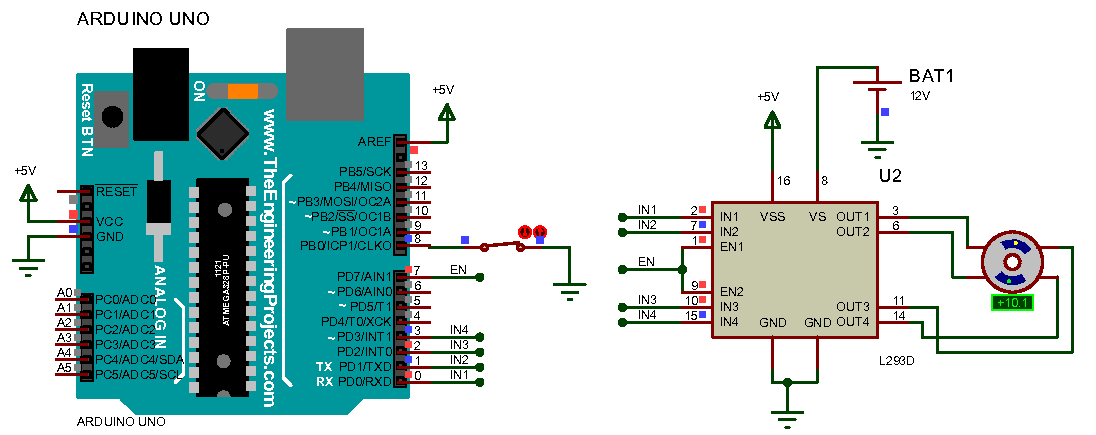
\includegraphics[scale=0.75]{Graphics/MICROS/Practice 1/ANIMATION/F10.PDF}
    }\fi
    
    \caption{Proteus Simulation}
    \label{fig:STEPPER_PROTEUS_ATMEGA}
\end{figure}


\clearpage












